\section{User Interface Design}

\begin{figure}[h]
    \centering
    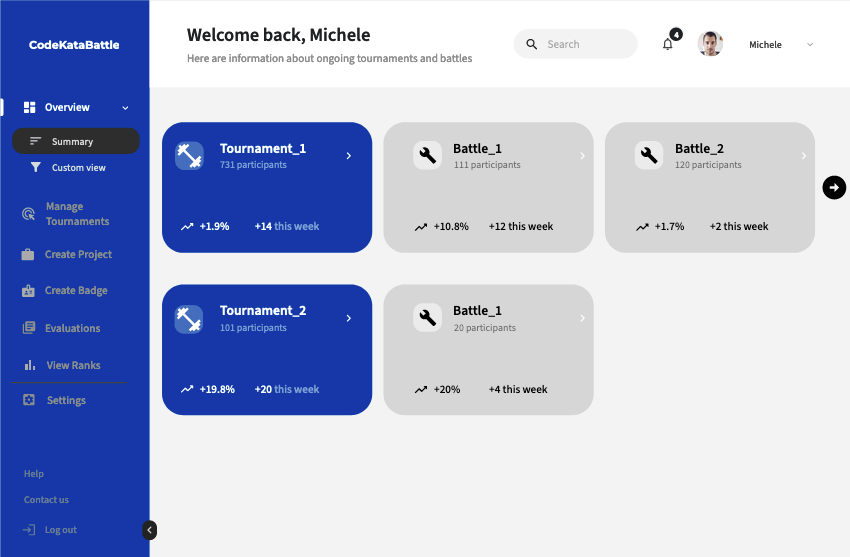
\includegraphics[scale=0.5]{src/educator_view.png}
    \caption*{Educator Interface}
\end{figure} \vspace{0.5cm}

In the Educator Interface the main page shows the ongoing tournaments, followed by every ongoing battle for that tournament. \\The search bar allows educator to search for a nickname and find users associated to it, so that it's possible to visualize their profile. \\The main functions an educator can perform are shown on the left column: 
\begin{itemize}
    \item \textbf{Manage Tournaments}: allows an educator to create and close a tournament, create (with all the possible settings) and close battles and eventually grant the permission to create battles to another educator.
    \item \textbf{Create Project}: allows an educator to create a new project to assign to students. 
    \item \textbf{Create Badge}: allows an educator to create a new badge that could be achieved by the students in a tournament.
    \item \textbf{Evaluations}: allows an educator to manually evaluate students' projects.
    \item \textbf{View Ranks}: view all ongoing tournaments and battles rank.
\end{itemize}

\vspace{100pt}

\begin{figure}[H]
    \centering
    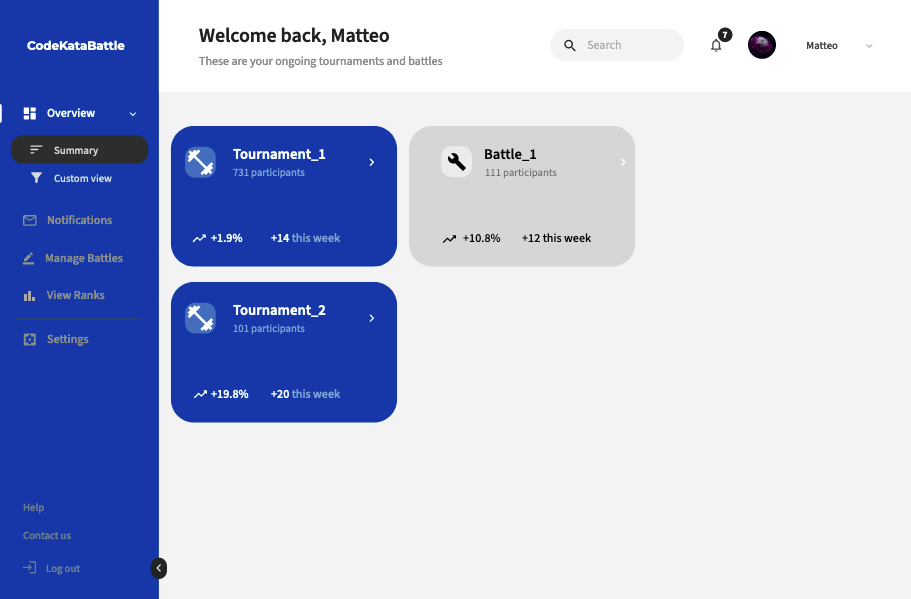
\includegraphics[scale=0.45]{src/student_view.png}
    \caption*{Student Interface}
\end{figure} \vspace{0.5cm}

In the Student Interface the main page shows the ongoing tournaments, followed by the battles to which the student is subscribed. \\The search bar allows student to search for a nickname and find users associated to it, so that it's possible to visualize their profile. \\The main functions a student can perform are shown on the left column:
\begin{itemize}
    \item \textbf{Notifications}: allows a student to view the notifications the platform sends when a new tournament or a new battle within a tournament the student is subscribed to is created.
    \item \textbf{Manage Battles}: this section allows a student to create teams and contains the link to the GitHub repository for each battles he/she is subscribed to. 
    \item \textbf{View Ranks}: view all ongoing tournaments and battles rank.
\end{itemize}
